\section{Product Data}
\paragraph{}Each time \app{} generates two XML-Configuration files. One for test configuration and another one for the tester's username and password. The ``-batch" (for configuration file) and ``-login-data" (for testers login information) endings will be added automatically into the names of the files.

\subsection{Configuration data}
\begin{description}
\item[/D010/ country]\hfill \\ Tester have to choose a country from the list of countries for testing. The chosen one will be added automatically into the all needed places in the XML-File.
\item[/D020/ URL]\hfill \\ Tester have to enter the URL for testing. The entered URL will be added automatically into the all needed places in the XML-File.
\item[/D030/ customer-number]\hfill \\ It is a number of a test customer account and necessary for testing.
\item[/D040/ tariff]\hfill \\ Tester have to enter the required tariff information for testing. The entered information will be added automatically into the all needed places in the XML-File.
\item[/D050/ tariff-addons]\hfill \\ Tester can enter the additional tariff options for testing (optional). The entered data will be added automatically into the all needed places in the XML-File.
\item[/D060/ domain]\hfill \\ Tester have to enter the domain for testing. The format looks like ``yourdomain.de". A time stamp will be added automatically before the last dot. The entered data will be edited in background automatically and automatically into the needed place in form ``yourdomain\{TIMESTAMP\}.de"  in the XML-File.
\item[/D070/ domain-bundle]\hfill \\ Tester can set the domain-bundle option to the true or false (default is false) for testing (optional). The data will be added automatically into the needed place in the XML-File.
\end{description}

\begin{landscape}
\paragraph{Example of a generated XML-Configuration file:}
\begin{verbatim}
<?xml version="1.0"?>
<telesales-buying-agent-batch>
  <telesales-urls>
    <telesales-url country="DE">https://hosting-ts-de.ts-host.gem1.sales.united.domain:9613/</telesales-url>
    <telesales-url country="ES">https://hosting-ts-es.ts-host.gem1.sales.united.domain:9613/</telesales-url>
    <telesales-url country="FR">https://hosting-ts-fr.ts-host.gem1.sales.united.domain:9613/</telesales-url>
    …
  </telesales-urls>
  <customers>
    <customer country="DE">
      <customer-number>7156019</customer-number>
    </customer>
    <customer country="FR">
      <customer-number>207958780</customer-number>
    </customer>
    …
  </customers>
  <orders>
    <order>
      <country>DE</country>
      <tariff>tariff-basic</tariff>
      <tariff-campaign-control>tariff-toggle</tariff-campaign-control>
      <tariff-addons>
        <tariff-addon id="presales.articles.slot-eshop-addon">opt-addon-eshop-basic</tariff-addon>
        <tariff-addon id="presales.articles.slot-sitelock-basic-addon">opt-addon-sitelock-basic</tariff-addon>
        <tariff-addon id="presales.articles.slot-seotool-addon">opt-addon-seotool</tariff-addon>
        …
      </tariff-addons>
      <domain>deinedomain{TIMESTAMP}.de</domain> <!-- {TIMESTAMP} will be replaced by yyyyMMddHHmmss -->
      <domain-bundle>false</domain-bundle>
    </order>
    <order>
      <country>FR</country>
      <tariff>tariff-basic</tariff>
      <tariff-campaign-control>tariff-toggle</tariff-campaign-control>
      <tariff-addons />
      <domain>votredomain{TIMESTAMP}.fr</domain> <!-- {TIMESTAMP} will be replaced by yyyyMMddHHmmss -->
      <domain-bundle>true</domain-bundle>
    </order>
  </orders>
</telesales-buying-agent-batch>
\end{verbatim}

\begin{figure}[h!]
\centering
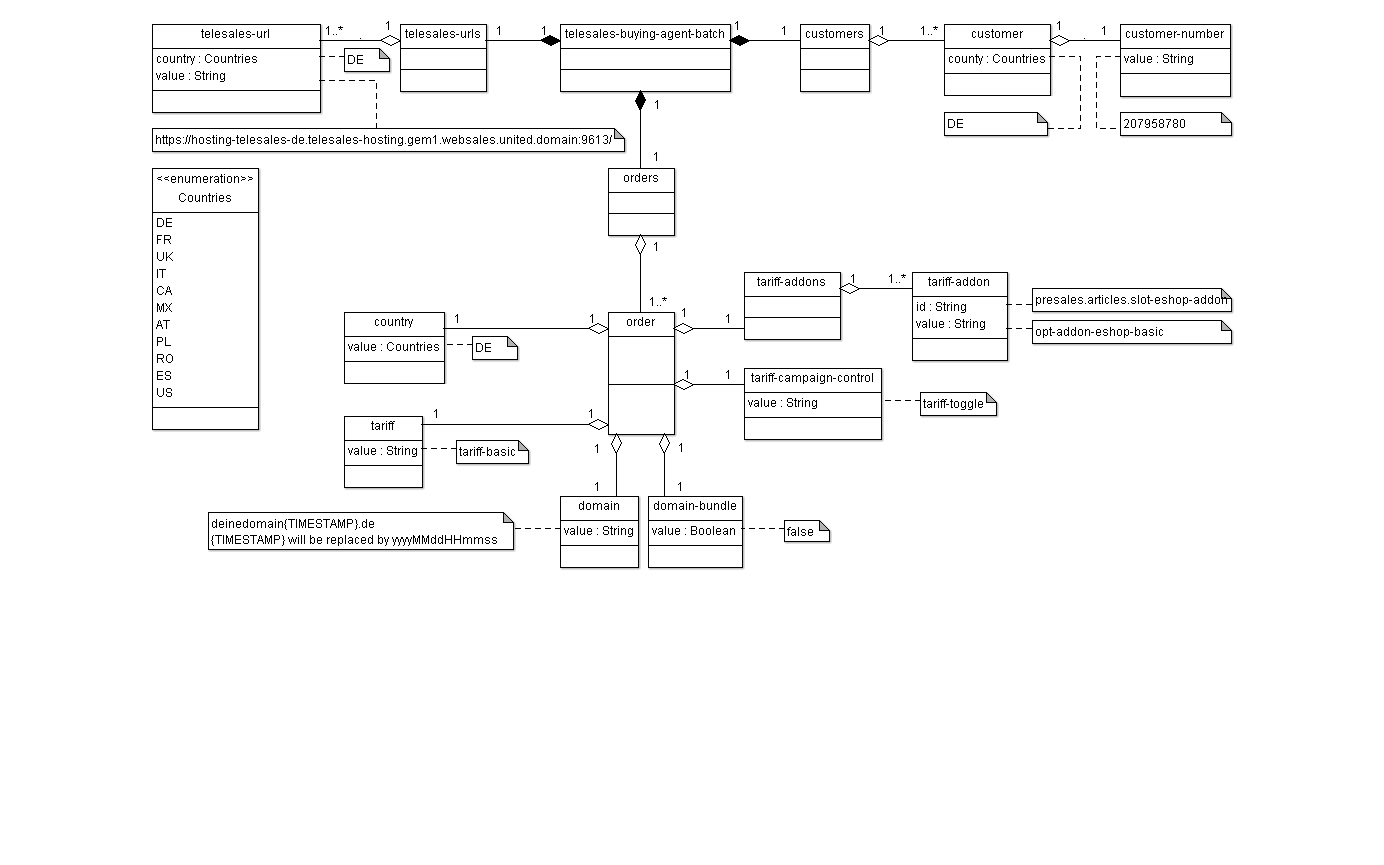
\includegraphics[width=1.1\textwidth]{d_class_batch.png}
\caption{UML Class diagramm of the Configuration file}
\end{figure}

\end{landscape}

\subsection{Login data}
\paragraph{}This data will be used as a login data of the testers.
\begin{description}
\item[/DC010/ username]\hfill\\ Tester's username.
\item[/DC020/ password]\hfill\\ Tester's password.
\end{description}

\paragraph{Example of a generated XML-Login-data file:}
\begin{verbatim}
<?xml version="1.0"?>
<telesales-buying-agent-login-data>
    <username>DeinBenutzername</username>
    <password>DeinPasswort</password>
</telesales-buying-agent-login-data>
\end{verbatim}

\begin{figure}[h!]
\centering
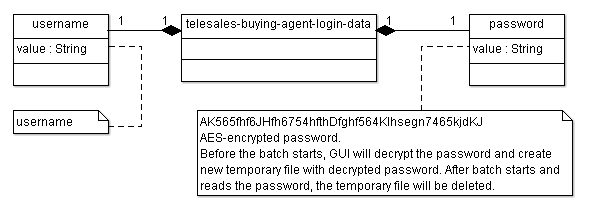
\includegraphics[width=\textwidth]{d_class_login-data.png}
\caption{UML Class diagramm of the Login data file}
\end{figure}
